\documentclass{standalone}
\usepackage{tikz}
\usetikzlibrary{patterns, positioning}
\usepackage[sfdefault]{ClearSans} %% option 'sfdefault' activates Clear Sans as the default text font
\usepackage[T1]{fontenc}

\begin{document}
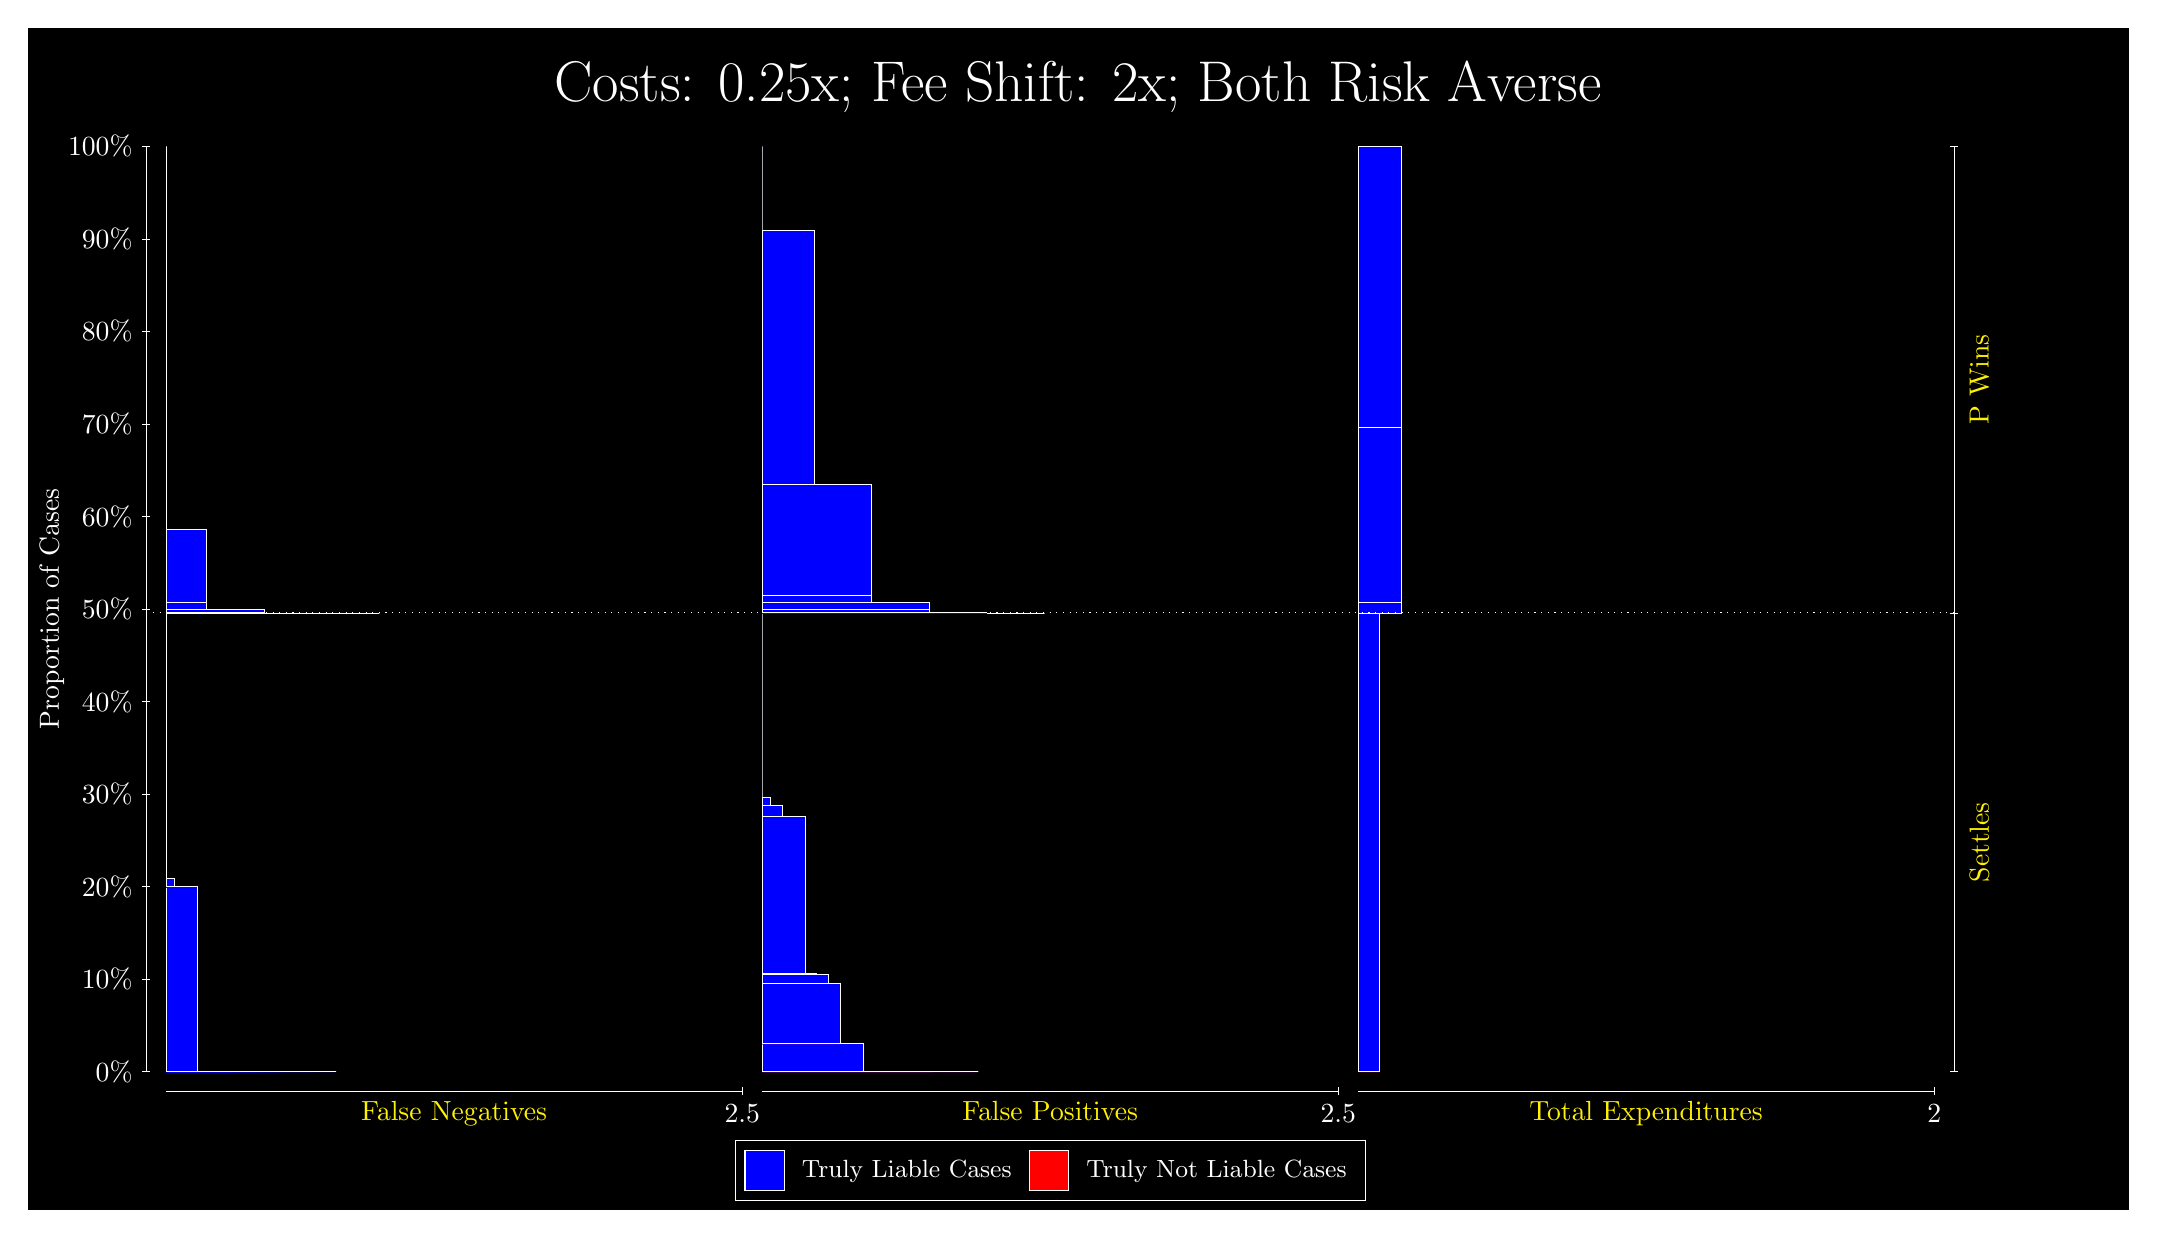
\begin{tikzpicture}
\draw[fill=black] (0,0) rectangle (26.667,15);
\draw[text=white] (0,13.5) rectangle (26.667,15) node[midway] {\huge Costs: 0.25x; Fee Shift: 2x; Both Risk Averse};
\draw[white, very thin] (1.5,1.75) -- (1.5,13.5);
\node[rotate=90, text=white, anchor=center] at (0.3, 7.625) {Proportion of Cases};
\draw[white, very thin] (1.45,1.75) -- (1.55,1.75);
\node[text=white, anchor=east] at (1.45, 1.75) {0\%};
\draw[white, very thin] (1.45,2.925) -- (1.55,2.925);
\node[text=white, anchor=east] at (1.45, 2.925) {10\%};
\draw[white, very thin] (1.45,4.1) -- (1.55,4.1);
\node[text=white, anchor=east] at (1.45, 4.1) {20\%};
\draw[white, very thin] (1.45,5.275) -- (1.55,5.275);
\node[text=white, anchor=east] at (1.45, 5.275) {30\%};
\draw[white, very thin] (1.45,6.45) -- (1.55,6.45);
\node[text=white, anchor=east] at (1.45, 6.45) {40\%};
\draw[white, very thin] (1.45,7.625) -- (1.55,7.625);
\node[text=white, anchor=east] at (1.45, 7.625) {50\%};
\draw[white, very thin] (1.45,8.8) -- (1.55,8.8);
\node[text=white, anchor=east] at (1.45, 8.8) {60\%};
\draw[white, very thin] (1.45,9.975) -- (1.55,9.975);
\node[text=white, anchor=east] at (1.45, 9.975) {70\%};
\draw[white, very thin] (1.45,11.15) -- (1.55,11.15);
\node[text=white, anchor=east] at (1.45, 11.15) {80\%};
\draw[white, very thin] (1.45,12.325) -- (1.55,12.325);
\node[text=white, anchor=east] at (1.45, 12.325) {90\%};
\draw[white, very thin] (1.45,13.5) -- (1.55,13.5);
\node[text=white, anchor=east] at (1.45, 13.5) {100\%};

\draw[white, very thin] (24.457,1.75) -- (24.457,13.5);
\draw[white, very thin] (24.407,1.75) -- (24.507,1.75);
\node[anchor=west] at (24.407, 1.75) {};
\draw[white, very thin] (24.407,7.5759) -- (24.507,7.5759);
\node[anchor=west] at (24.407, 7.5759) {};
\draw[white, very thin] (24.407,13.5) -- (24.507,13.5);
\node[anchor=west] at (24.407, 13.5) {};

\draw[white, very thin, fill=blue] (1.75,1.75) rectangle (3.9091,1.75);
\draw[white, very thin, fill=blue] (1.75,1.75) rectangle (3.6163,1.75);
\draw[white, very thin, fill=blue] (1.75,1.75) rectangle (3.3236,1.75);
\draw[white, very thin, fill=blue] (1.75,1.75) rectangle (3.1772,1.75);
\draw[white, very thin, fill=blue] (1.75,1.75) rectangle (3.0308,1.75);
\draw[white, very thin, fill=blue] (1.75,1.75) rectangle (2.8844,1.75);
\draw[white, very thin, fill=blue] (1.75,1.75) rectangle (2.738,1.75);
\draw[white, very thin, fill=blue] (1.75,1.75) rectangle (2.5917,1.7502);
\draw[white, very thin, fill=blue] (1.75,1.7502) rectangle (2.4453,1.7508);
\draw[white, very thin, fill=blue] (1.75,1.7508) rectangle (2.2989,1.7508);
\draw[white, very thin, fill=blue] (1.75,1.7508) rectangle (2.1525,4.0974);
\draw[white, very thin, fill=blue] (1.75,4.0974) rectangle (2.0062,4.0985);
\draw[white, very thin, fill=blue] (1.75,4.0985) rectangle (1.8598,4.1999);
\draw[white, very thin, fill=red] (1.75,4.1999) rectangle (1.75,4.1999);
\draw[white, very thin, fill=blue] (1.75,4.1999) rectangle (1.75,7.5759);
\draw[white, very thin, fill=blue] (1.75,7.5759) rectangle (4.458,7.5759);
\draw[white, very thin, fill=blue] (1.75,7.5759) rectangle (3.7261,7.5761);
\draw[white, very thin, fill=blue] (1.75,7.5761) rectangle (2.9942,7.5762);
\draw[white, very thin, fill=blue] (1.75,7.5762) rectangle (2.9942,7.6266);
\draw[white, very thin, fill=blue] (1.75,7.6266) rectangle (2.2623,7.7155);
\draw[white, very thin, fill=blue] (1.75,7.7155) rectangle (2.2623,8.637);
\draw[white, very thin, fill=red] (1.75,8.637) rectangle (1.75,8.637);
\draw[white, very thin, fill=blue] (1.75,8.637) rectangle (1.75,13.5);
\draw[white, very thin, fill=red] (9.3189,1.75) rectangle (12.063,1.75);
\draw[white, very thin, fill=blue] (9.3189,1.75) rectangle (12.063,1.75);
\draw[white, very thin, fill=red] (9.3189,1.75) rectangle (11.478,1.75);
\draw[white, very thin, fill=blue] (9.3189,1.75) rectangle (11.478,1.75);
\draw[white, very thin, fill=blue] (9.3189,1.75) rectangle (11.332,1.752);
\draw[white, very thin, fill=red] (9.3189,1.752) rectangle (11.185,1.752);
\draw[white, very thin, fill=blue] (9.3189,1.752) rectangle (11.185,1.752);
\draw[white, very thin, fill=red] (9.3189,1.752) rectangle (10.892,1.752);
\draw[white, very thin, fill=blue] (9.3189,1.752) rectangle (10.892,1.7529);
\draw[white, very thin, fill=blue] (9.3189,1.7529) rectangle (10.746,1.7539);
\draw[white, very thin, fill=red] (9.3189,1.7539) rectangle (10.6,1.7539);
\draw[white, very thin, fill=blue] (9.3189,1.7539) rectangle (10.6,2.1036);
\draw[white, very thin, fill=blue] (9.3189,2.1036) rectangle (10.453,2.1038);
\draw[white, very thin, fill=red] (9.3189,2.1038) rectangle (10.307,2.1038);
\draw[white, very thin, fill=blue] (9.3189,2.1038) rectangle (10.307,2.8659);
\draw[white, very thin, fill=blue] (9.3189,2.8659) rectangle (10.161,2.9788);
\draw[white, very thin, fill=blue] (9.3189,2.9788) rectangle (10.014,3.0023);
\draw[white, very thin, fill=blue] (9.3189,3.0023) rectangle (9.8678,4.9896);
\draw[white, very thin, fill=blue] (9.3189,4.9896) rectangle (9.7214,4.9898);
\draw[white, very thin, fill=blue] (9.3189,4.9898) rectangle (9.575,5.126);
\draw[white, very thin, fill=blue] (9.3189,5.126) rectangle (9.4287,5.2274);
\draw[white, very thin, fill=blue] (9.3189,5.2274) rectangle (9.3189,7.5759);
\draw[white, very thin, fill=red] (9.3189,7.5759) rectangle (12.905,7.5759);
\draw[white, very thin, fill=blue] (9.3189,7.5759) rectangle (12.905,7.5759);
\draw[white, very thin, fill=blue] (9.3189,7.5759) rectangle (12.173,7.5768);
\draw[white, very thin, fill=red] (9.3189,7.5768) rectangle (12.173,7.5768);
\draw[white, very thin, fill=blue] (9.3189,7.5768) rectangle (12.173,7.5777);
\draw[white, very thin, fill=blue] (9.3189,7.5777) rectangle (11.441,7.6196);
\draw[white, very thin, fill=red] (9.3189,7.6196) rectangle (11.441,7.6196);
\draw[white, very thin, fill=blue] (9.3189,7.6196) rectangle (11.441,7.7146);
\draw[white, very thin, fill=blue] (9.3189,7.7146) rectangle (10.709,7.8023);
\draw[white, very thin, fill=red] (9.3189,7.8023) rectangle (10.709,7.8023);
\draw[white, very thin, fill=blue] (9.3189,7.8023) rectangle (10.709,9.2114);
\draw[white, very thin, fill=blue] (9.3189,9.2114) rectangle (9.9776,9.2139);
\draw[white, very thin, fill=red] (9.3189,9.2139) rectangle (9.9776,9.2139);
\draw[white, very thin, fill=blue] (9.3189,9.2139) rectangle (9.9776,12.439);
\draw[white, very thin, fill=blue] (9.3189,12.439) rectangle (9.3189,13.5);
\draw[white, very thin, fill=red] (16.888,1.75) rectangle (17.162,1.75);
\draw[white, very thin, fill=blue] (16.888,1.75) rectangle (17.162,7.5759);
\draw[white, very thin, fill=red] (16.888,7.5759) rectangle (17.437,7.5759);
\draw[white, very thin, fill=blue] (16.888,7.5759) rectangle (17.437,7.7089);
\draw[white, very thin, fill=red] (16.888,7.7089) rectangle (17.437,7.7089);
\draw[white, very thin, fill=blue] (16.888,7.7089) rectangle (17.437,9.9332);
\draw[white, very thin, fill=red] (16.888,9.9332) rectangle (17.437,9.9332);
\draw[white, very thin, fill=blue] (16.888,9.9332) rectangle (17.437,13.5);
\draw[white, dotted] (1.5,7.5759) -- (24.457,7.5759);
\draw[white, very thin] (1.75,1.5) -- (9.0689,1.5);
\node[text=yellow, anchor=north] at (5.4094, 1.5) {False Negatives};
\draw[white, very thin] (9.0689,1.45) -- (9.0689,1.55);
\node[text=white, anchor=north] at (9.0689, 1.45) {2.5};

\draw[white, very thin] (9.3189,1.5) -- (16.638,1.5);
\node[text=yellow, anchor=north] at (12.978, 1.5) {False Positives};
\draw[white, very thin] (16.638,1.45) -- (16.638,1.55);
\node[text=white, anchor=north] at (16.638, 1.45) {2.5};

\draw[white, very thin] (16.888,1.5) -- (24.207,1.5);
\node[text=yellow, anchor=north] at (20.547, 1.5) {Total Expenditures};
\draw[white, very thin] (24.207,1.45) -- (24.207,1.55);
\node[text=white, anchor=north] at (24.207, 1.45) {2};

\node[text=yellow, centered, rotate=90] at (24.777, 4.663) {Settles};
\node[text=yellow, centered, rotate=90] at (24.777, 10.538) {P Wins};

\draw (12.978300999999998,1.5) node[draw=none] (baseCoordinate) {};
\begin{scope}[align=center]
        \matrix[scale=0.5, draw=white, below=0.5cm of baseCoordinate, nodes={draw}, column sep=0.1cm]{
            \node[rectangle, draw, minimum width=0.5cm, minimum height=0.5cm, fill=blue] {}; &
            \node[draw=none, font=\small, text=white] (B) {Truly Liable Cases}; &
            \node[rectangle, draw, minimum width=0.5cm, minimum height=0.5cm, fill=red] {}; &
            \node[draw=none, font=\small, text=white] (B) {Truly Not Liable Cases}; \\
            };
\end{scope}

\end{tikzpicture}
\end{document}